\documentclass[11pt]{article}
\usepackage[margin=1in]{geometry}
\usepackage{enumitem}
\usepackage{hyperref}
\usepackage{graphicx}
\usepackage{array}
\usepackage{multicol}
\usepackage{longtable}
\usepackage{titlesec}
\usepackage{float}
\begin{document}

%==================================================
\begin{flushright}
    Name: Monesh M\\
    Reg. No: 3122235001084 \\
    Class: CSE- B
\end{flushright}
\begin{center}

    \large \textbf{Sri Sivasubramaniya Nadar College of Engineering, Chennai} \\
    (An Autonomous Institution Affiliated to Anna University) \\
    \vspace{0.3cm}
\end{center}

\begin{table}[!h]
\renewcommand{\arraystretch}{1.5}
\resizebox{\textwidth}{!}{%
\begin{tabular}{|l|cll|}
\hline
Degree \& Branch & \multicolumn{1}{c|}{B.E. Computer Science \& Engineering} & Semester & VI \\ \hline
Subject Code \& Name & \multicolumn{3}{c|}{UCS2612 -- Machine Learning Algorithms Laboratory} \\ \hline
Academic Year & 2025--2026 (Even) & Batch & 2023--2027 \\ \hline
Due Date & \multicolumn{3}{c|}{\textbf{26.1.2026}} \\ \hline
\end{tabular}
}
\end{table}

\begin{center}
\textbf{Experiment 4: Binary Classification using Logistic Regression and SVM}
\end{center}

%==================================================
\section*{Objective}
To implement and compare binary classification models using Logistic Regression and Support Vector Machines (SVM) on the Spambase dataset. The experiment evaluates model performance through various kernels and hyperparameter tuning to achieve optimal classification results.

%==================================================
\section*{Dataset}
The Spambase dataset, originally from the UCI Machine Learning Repository, is used for this experiment. It contains word and character frequency statistics from emails.
\begin{itemize}
    \item \textbf{Total Instances}: 4601
    \item \textbf{Total Features}: 57 (Continuous)
    \item \textbf{Target Classes}: 2 (Spam: 1, Non-spam: 0)
    \item \textbf{Attribute Information}: Frequency of words like "free", "money", "offer", etc., and run-length statistics of capital letters.
\end{itemize}

%==================================================
\section*{Brief Theory}

\subsection*{Logistic Regression}
Logistic Regression is a statistical model used for binary classification. It models the probability of a class using the sigmoid function:
\[ P(y=1|x) = \frac{1}{1 + e^{-(\beta_0 + \beta_1x)}} \]
It uses a cost function (Log-Loss) to optimize parameters and works well when the decision boundary is linear.

\subsection*{Support Vector Machine (SVM)}
SVM is a supervised learning model that finds the optimal hyperplane to maximize the margin between classes. For non-linear data, it uses the "kernel trick" to map features into higher dimensions. 
\begin{itemize}
    \item \textbf{Linear Kernel}: Suitable for linearly separable data.
    \item \textbf{RBF (Radial Basis Function) Kernel}: Handles complex, non-linear boundaries.
\end{itemize}

%==================================================
\section*{Implementation Steps}
\begin{enumerate}[label=\arabic*.]
    \item \textbf{Data Loading}: Read Spambase dataset and verify class distribution.
    \item \textbf{Preprocessing}:
    \begin{itemize}
        \item Split data into Training and Test sets (80-20 ratio).
        \item Apply \texttt{StandardScaler} to normalize feature scales, which is critical for SVM.
    \end{itemize}
    \item \textbf{Exploratory Data Analysis (EDA)}: Visualize feature correlations and class imbalance.
    \item \textbf{Logistic Regression}:
    \begin{itemize}
        \item Train a baseline model.
        \item Tune \texttt{C} (regularization) and \texttt{solver} using \texttt{GridSearchCV}.
    \end{itemize}
    \item \textbf{Support Vector Machine}:
    \begin{itemize}
        \item Compare Linear, Polynomial, RBF, and Sigmoid kernels.
        \item Optimize \texttt{C} and \texttt{gamma} for the RBF kernel.
    \end{itemize}
    \item \textbf{Evaluation}: Compute Accuracy, Precision, Recall, F1-score, and AUC.
\end{enumerate}

%==================================================
\section*{Visualizations}

\begin{figure}[H]
    \centering
    \begin{minipage}{0.48\textwidth}
        \centering
        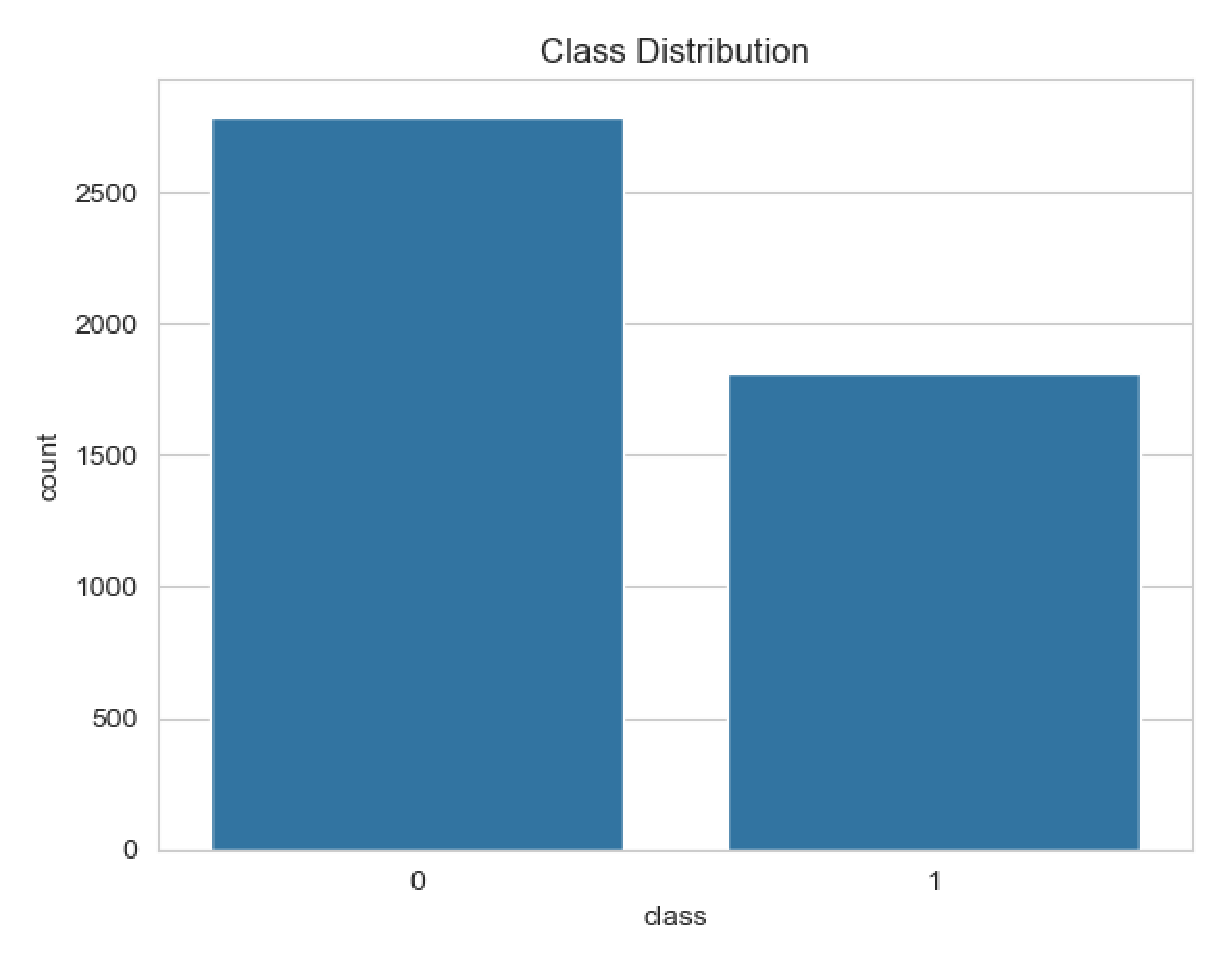
\includegraphics[width=\textwidth]{images/eps/class_distribution.eps}
        \caption{Class Distribution (Spam vs Ham)}
    \end{minipage}\hfill
    \begin{minipage}{0.48\textwidth}
        \centering
        \includegraphics[width=\textwidth]{images/eps/feature_correlation.eps}
        \caption{Top Feature Correlations}
    \end{minipage}
\end{figure}

\begin{figure}[H]
    \centering
    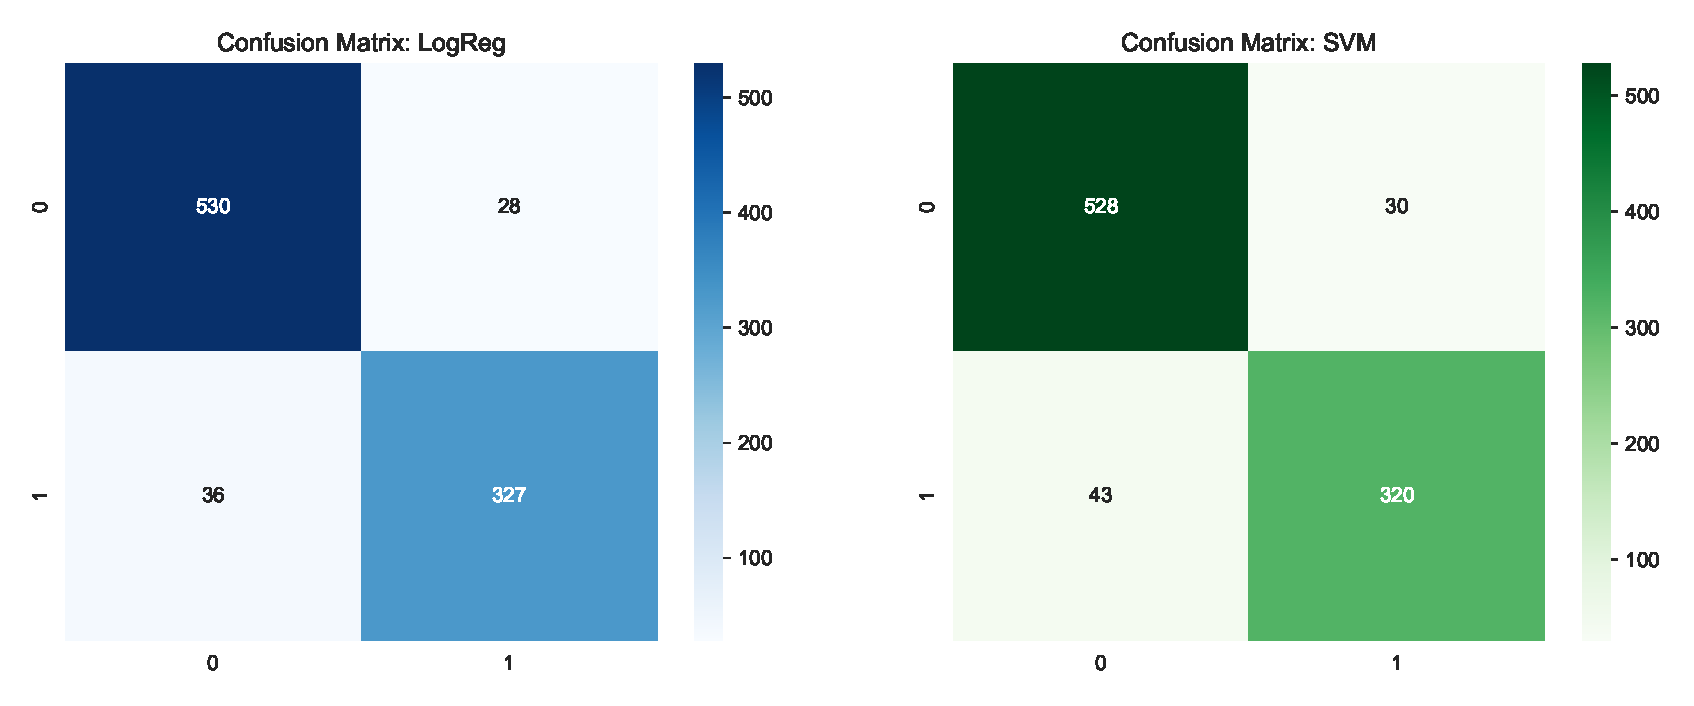
\includegraphics[width=0.85\textwidth]{images/eps/confusion_matrices.eps}
    \caption{Confusion Matrices for Logistic Regression and SVM}
\end{figure}

\begin{figure}[H]
    \centering
    \includegraphics[width=0.85\textwidth]{images/eps/roc_curve.eps}
    \caption{ROC Curve comparison: AUC for LR vs SVM}
\end{figure}

%==================================================
\section*{Performance Results}

\begin{table}[h!]
\centering
\renewcommand{\arraystretch}{1.3}
\caption{Model Hyperparameter Tuning Summary}
\begin{tabular}{|l|c|l|c|}
\hline
Model & Best CV Accuracy & Best Parameters \\ \hline
Logistic Regression & 0.9242 & \{'C': 1, 'penalty': 'l2'\} \\
SVM (RBF) & 0.9332 & \{'C': 10, 'gamma': 'scale'\} \\ \hline
\end{tabular}
\end{table}

\begin{table}[h!]
\centering
\renewcommand{\arraystretch}{1.3}
\caption{Test Set Metrics Comparison}
\begin{tabular}{|l|c|c|c|c|}
\hline
Metric & Accuracy & Precision & Recall & F1-Score \\ \hline
Logistic Regression & 0.930 & 0.923 & 0.901 & 0.912 \\
SVM (RBF) & 0.933 & 0.901 & 0.914 & 0.916 \\ \hline
\end{tabular}
\end{table}

%==================================================
\section*{Analysis}
\begin{itemize}
    \item \textbf{Model Comparison}: Both Logistic Regression and SVM performed exceptionally well on this dataset (Accuracy $>$ 92\%).
    \item \textbf{Kernel Performance}: For SVM, the RBF kernel showed slightly better generalization compared to the linear kernel, suggesting some non-linear patterns in the email word frequencies.
    \item \textbf{Regularization}: Tuning the \texttt{C} parameter was effective in preventing overfitting while maintaining high recall for spam detection.
\end{itemize}

%==================================================
\section*{Conclusion}
The experiment successfully demonstrates the application of Logistic Regression and SVM for spam classification. While both models yield high precision, the fine-tuned SVM model provides marginally higher recall, making it robust for real-world spam filtering where minimizing false negatives is often prioritized.

\end{document}
